\documentclass[../main.tex]{subfiles}
\graphicspath{{\subfix{../figures/}}}

\begin{document}
\section{UML 中的静态图}
\textbf{静态建模}:
任何建模语言都以静态建模机制为基础,标准建模语言UML也不例外.所谓静态建模是指建立系统内部结构及各部分之间的互相联系,而这些关系不随时间而转移.
\textbf{类和对象的建模},是UML静态建模的主要内容,也是UML建模的基础.
\subsection{类图}
类图(Class Diagram)描述类和类之间的静态关系.与数据模型不同,它不仅显示了信息的结构,同时还描述了系统的行为.类图是定义其它图的基础.
\begin{figure}[H]
  \begin{center}
    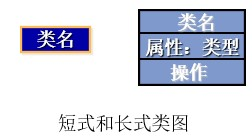
\includegraphics[width=0.25\textwidth]{5_1.jpg}
  \end{center}
\end{figure}
\textbf{类图的结构}:类图表示为一个划分成三个格子的长方形.
类及类型名均用英文大写字母开头,属性及操作名为小写字母开头.
\begin{itemize}
  \item \textbf{类名}
  \item \textbf{属性}(可见性, 名称, 类型, 缺省值和约束特性)
    \begin{itemize}
      \item \textbf{属性书写的语法}: 可见性 属性名 :类型 = 缺省值 \{约束特性\}
      \item \textbf{可见性}:``+'': Public, ``-'': Private, ``\#'': Protected.
      \item \textbf{约束}:是用户对该属性性质一个约束的说明.e.g. \{只读\}
    \end{itemize}
  \item \textbf{方法}书写语法:可见性 操作名(参数表):返回类型 \{约束特性\}
\end{itemize}
\textbf{使用类图的几个建议}
\begin{itemize}
  \item 不要试图使用所有的符号.
  \item 根据项目开发的不同阶段,用正确的观点来画类图.
  \item 不要为每个事物都画一个模型,应该把精力放在关键的领域.
  \item 当用一张A4纸不足以容纳所有的类图时,就应该用包图.
\end{itemize}
\textbf{类间的关系}:
\begin{figure}[H]
  \begin{center}
    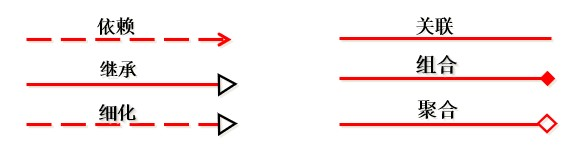
\includegraphics[width=0.55\textwidth]{5_2.jpg}
  \end{center}
\end{figure}
\textbf{类图的层次}:类图的抽象层次和细化(Refinement)关系-在需求分析阶段,类图是研究问题领域的概念;在设计阶段,类图描述类与类之间的接口;而在实现阶段,类图描述软件系统中类的实现.
\begin{itemize}
  \item \textbf{概念层}(Conceptual)类图描述应用领域中的概念.
  \item \textbf{说明层}(Specification)类图描述软件的接口部分,而不是软件的实现部分.
  \item 只有在\textbf{实现层}(Implementation)才真正有类的概念,并且揭示软件的实现部分.
\end{itemize}
\textbf{细化关系}:有两个元素A和B,若B元素是A元素的更详细描述,则称为B元素细化A元素(B
$ \rightarrow $ A).
细化与类的抽象层次有密切的关系,在构造模型时要经过逐步细化,逐步求精的过程.

\textbf{关联和链}:关联(association)是两个或多个独立类之间固有的关系.链(link)是关联的具体体现.
关联分为二元关联(binary), 三元关联(ternary), 多元关联(higher order).
\begin{figure}[H]
  \begin{center}
    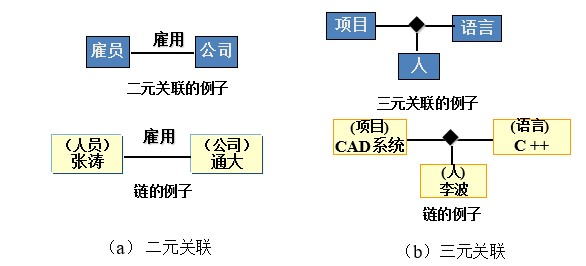
\includegraphics[width=0.55\textwidth]{5_3.jpg}
  \end{center}
\end{figure}
\textbf{关联的重数}:重数(multiplicity)表示多少个对象参与到关联关系中,重数的默认值为 $ 1 $.
常用重数符号有:
\begin{itemize}
  \item  ``0..1'':表示0或1
  \item  ``0..*'' 或 ``*'':表示0或多个
  \item  ``1..*'':表示1或多个
  \item  ``1,3,7'':表示 $ 1 $ 或 $ 3 $ 或 $ 7 $(枚举型)
\end{itemize}
\begin{figure}[H]
  \begin{center}
    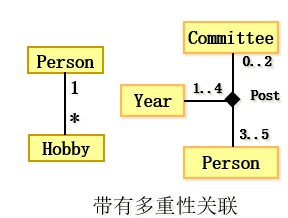
\includegraphics[width=0.35\textwidth]{5_4.jpg}
  \end{center}
\end{figure}
\noindent \textbf{有序关联与导航(导引)}:
在关联的多端标注\{ordered\}指明这些类之间的关系是有序的.
关联可以用箭头,表示该关联关系的方向(单向或双向),称为导引或导航(navigation).
\begin{figure}[H]
  \begin{center}
    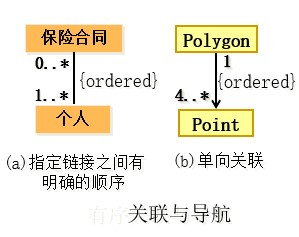
\includegraphics[width=0.35\textwidth]{5_5.jpg}
  \end{center}
\end{figure}
\noindent \textbf{依赖}:依赖关系描述的是两个模型元素(类,组合,用例等)之间的使用与被使用的关系,其中一个模型元素是独立的,另一个模型元素是非独立的(或依赖的).如图表示类A依赖于类B的一个友元依赖关系.
\begin{figure}[H]
  \begin{center}
    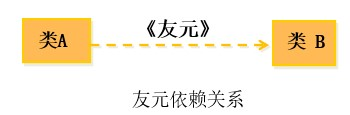
\includegraphics[width=0.25\textwidth]{5_6.jpg}
  \end{center}
\end{figure}
\noindent 依赖的形式可能是多样的,针对不同的依赖的形式,依赖关系有不同的变体(varieties):如友元、访问、调用、创建等.
\subsection{对象图}
\noindent 对象与类的图形表示相似,为划分成两个格子的长方形(对象名和属性值).
对象图是类图的一种实例化.一张对象图表示的是与其对应的类图的一个具体实例,
即系统在某一时期或者某一特定时刻可能存在的具体对象实例以及它们相互之间的具体关系.
\subsection{包图}
\noindent \textbf{为何引入包(Package)}:降低系统的复杂性.

\noindent \textbf{什么是UML包}:
是将许多类集合成一个更高层次的单位,形成一个高内聚、低耦合的类的集合;
是一种分组机制,把各种各样的模型元素通过内在的语义连接为一个整体;
构成包的模型元素称为包的内容,包通常用于对模型的组织管理,因此有时又将包称为子系统(subsystem).
\begin{figure}[H]
  \begin{center}
    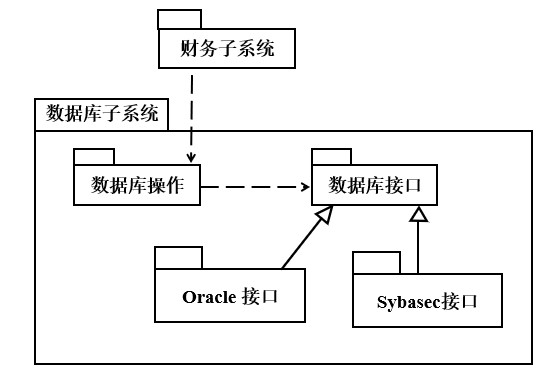
\includegraphics[width=0.40\textwidth]{5_7.jpg}
  \end{center}
\end{figure}
\noindent \textbf{包的内容}:可以是类的列表,也可以是另一个包图,还可以是一个类图.

\noindent \textbf{包之间的关系}:
\begin{itemize}
  \item \textbf{依赖关系}:两个包中的任意两个类存在依赖关系,则包之间存在依赖关系.
  \item \textbf{泛化关系}:使用继承中一般和特殊的概念来说明通用包和专用包之间的关系.例如,专用包必须符合通用包的接口,与类继承关系类似.
\end{itemize}
\textbf{包图的表示}:
\begin{figure}[H]
  \begin{center}
    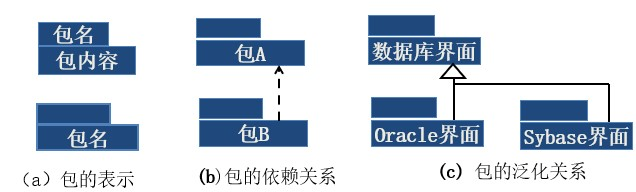
\includegraphics[width=0.45\textwidth]{5_8.jpg}
  \end{center}
\end{figure}
\begin{figure}[H]
  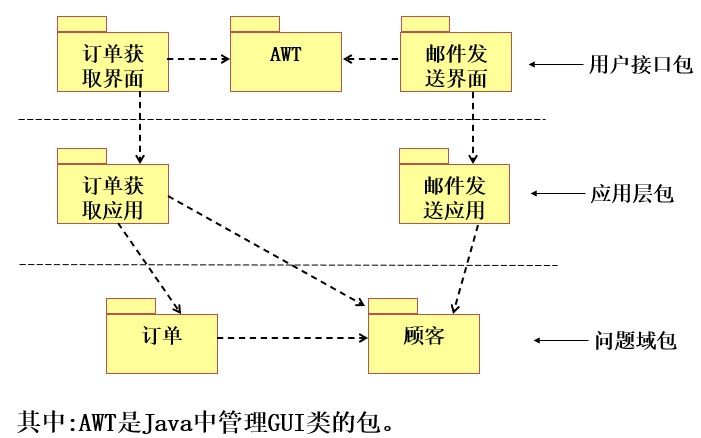
\includegraphics[width=0.50\textwidth]{5_9.jpg}
    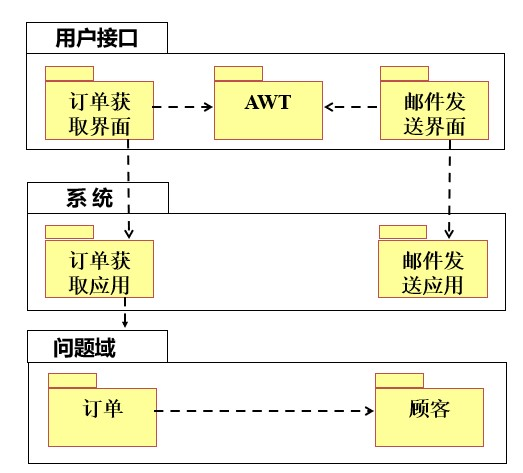
\includegraphics[width=0.50\textwidth]{5_10.jpg}
\end{figure}
\noindent \textbf{类的识别}:是面向对象方法的一个难点,但又是建模的关键.常用方法有:
\begin{enumerate}
  \item \textbf{名词识别法}
  \item \textbf{系统实体识别法}
  \item \textbf{从用例中识别类}:根据用例的描述来识别类
    \begin{itemize}
      \item 用例的描述中出现哪些实体?
      \item 用例执行过程中产生并存储哪些信息?
      \item 与用例关联的角色向用例输入什么信息?
      \item 用例又向该角色输出哪些信息?
    \end{itemize}
  \item \textbf{利用分解与抽象技术}
    \begin{itemize}
      \item 分解技术:将整体类和组合类分解.可控制单个类的规模.
      \item 抽象技术:根据一些类的相似性建立抽象类,并建立抽象类与这些类之间的继承关系.
      \item 抽象类实现了系统内部的重用,很好地控制了复杂性,并为所有子类定义了一个公共的接口,使设计局部化,提高系统的可修改性和可维护性.
    \end{itemize}
\end{enumerate}
关键是要定义类的属性及操作. \\
\textbf{名词识别法}:识别问题域中的实体,实体的描述通常用名词、名词短语、名词性代词的形式出现.
\begin{itemize}
  \item 用指定语言对系统进行描述;描述过程应与领域专家共同合作完成,并遵循问题域中的概念和命名.
  \item 从系统描述中标识名词、名词短语、名词性代词;识别确定(取、舍)类.
    为了发现对象和类,开发人员要在系统需求和系统分析的文档中查找名词和名词短语,包括:可感知的事物、角色、事件、互相作用、人员、场所、组织、设备和地点等.
  \item 对类进行筛选,根据下述原则进一步确定类:
    \begin{enumerate}
      \item 去掉冗余类:如两个类表述同一信息,应保留最具有描述能力的类.
      \item 去掉不相干的类:删除与问题无关或关系不大的类.
      \item 删除模糊的类或性质独立性不强的类:有些初始类边界定义不确切,或范围太广,应该删除.
      \item 所描述的操作不适宜作为对象类,所描述的只是实现过程中的暂时的对象,应删去.
    \end{enumerate}
\end{itemize}
\noindent \textbf{系统实体识别法}:不关心系统的运作流程及实体之间的通信状态,而只考虑系统中的人员、设备、组织、地点、表格、报告等实体,经过分析将他们识别为类(或对象).

\noindent \textbf{被标识的实体有}:
系统需要存储、分析、处理的信息实体;
系统内部需要处理的设备;
与系统交互的外部系统;
系统相关人员;
系统的组织实体.

\noindent \textbf{确定关联}:使用下列标准去掉不必要和不正确的关联
\begin{enumerate}
  \item 若某个类已被删除,那么与它有关的关联也必须删除或者用其他类来重新表述。
  \item 不相干的关联或实现阶段的关联。删除所有问题域之外的关联或涉及实现结构中的关联,
  \item 动作。关联应描述应用域的结构性质而不是瞬时事件。
  \item 派生关联,省略那些可以用其他关联来定义的关联,因为这种关联是冗余的。
\end{enumerate}
\subsection{医院病房监护系统}
\noindent 为了对危重病人进行实时监护,随时了解病人病情,及时进行处理,建立病房监护系统。  
病症监视器安置在每个病床,通过网络将病人的组合病症信号实时传送到中央监护系统进行分析处理。
在中心值班室里,值班护士使用中央监护系统对病员的情况进行监控,监护系统实时地将病人的病症信号与标准的病诊信号进行比较分析,当病症出现异常时,系统会立即自动报警,并打印病情报告和更新病历。
系统根据医生的要求随时打印病人的病情报告,系统定期自动更新病历。

经过初步的需求分析,得到系统功能要求:
\begin{enumerate}
  \item 监视病员的病症(血压、体温、脉搏等)
  \item 定时更新病历
  \item 病员出现异常情况时报警。
  \item 随机地产生某一病员的病情报告。
\end{enumerate}
通过名词识别法和系统实体识别法等方法可以确定系统的十二个类:
\begin{figure}[H]
    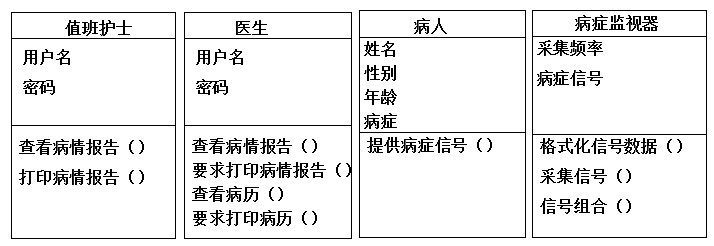
\includegraphics[width=0.50\textwidth]{5_11.jpg}
    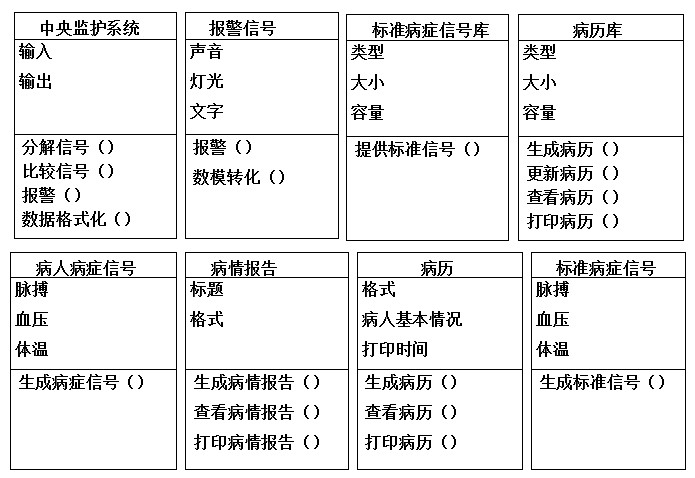
\includegraphics[width=0.50\textwidth]{5_12.jpg}
\end{figure}
\begin{figure}[H]
    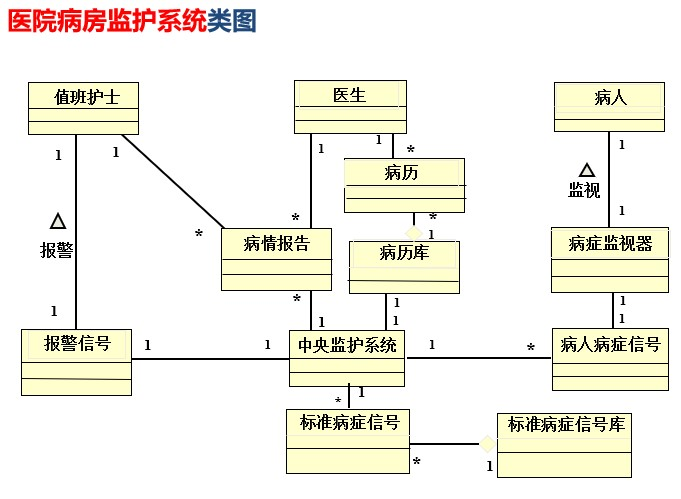
\includegraphics[width=0.60\textwidth]{5_13.jpg}
\end{figure}
\end{document}
